% -*- coding: utf-8 -*-

\chapter{状態空間問題 (State-Space Problem)}
\label{ch:state-space-problem}

% This chapter is ...
この章ではまず、\ref{sec:state-space-problem}節ではグラフ探索手法が用いられる問題として状態空間問題を定義する。
次に\ref{sec:search-problem}節で状態空間問題の例をいくつか紹介する。
経路探索問題や倉庫番問題など、応用がありつつ、かつ分かりやすい問題を選んだ。これらの問題はすべてヒューリスティック探索研究でベンチマークとして広く使われているものである。

\ref{sec:state-space-problem}節における定式化は\cite{russelln03}、\cite{pearl84}、\cite{edelkamp:2010:hst:1875144}などを参考にしている。本文は入門の内容であるので、研究の詳細が知りたい方はこれらの教科書を読むべきである。

%\captionlistentry[todo]{状態空間問題の例示}

\section{状態空間問題 (State-Space Problem)}
\label{sec:state-space-problem}

この本では主に初期状態とゴール条件が与えられたとき、ゴール条件を満たすための経路を返す問題を探索する手法を考える。
特に本書の主眼は\ref{ch:state-space-problem}章から\ref{ch:heuristic-search-variants}章までで扱う\define{状態空間問題}{state-space problem}{じょうたいくうかんもんだい}である。

\ddef{ユニットコスト状態空間問題、unit-cost state-space problem}{
	ユニットコスト状態空間問題$P_{u} = (S, A, s_0, T)$は状態の集合$S$、アクション集合$A = {a_1, ....,a_n}$、$a_i : S \rightarrow S$、初期状態$s_0 \in S$、ゴール集合$T \in S$、が与えられ、初期状態$s_0$からゴール状態のいずれかへ遷移させるアクションの列を返す問題である。
}

% \TODO{状態空間問題の例。それをグラフ問題に帰着させる例。}

\begin{figure}[htb]
  \centering
  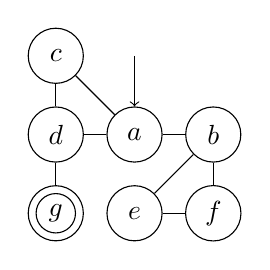
\begin{tikzpicture}[scale=0.5]
    % MDP i
\node [draw, circle, minimum size=0.7cm] (a) at (2, 2) {$a$};
\node [draw, circle, minimum size=0.7cm] (b) at (4, 2) {$b$};
\node [draw, circle, minimum size=0.7cm] (c) at (0, 4) {$c$};
\node [draw, circle, minimum size=0.7cm] (d) at (0, 2) {$d$};
\node [draw, circle, minimum size=0.7cm] (e) at (2, 0) {$e$};
\node [draw, circle, minimum size=0.7cm] (f) at (4, 0) {$f$};
\node [draw, circle, minimum size=0.7cm] (g) at (0, 0) {$g$};
\node [draw, circle, minimum size=0.5cm] at (0, 0) {};

\coordinate[above of=a] (init);

\draw[->] (init) -- (a);
\draw[-] (a) -- (b);
\draw[-] (a) -- (c);
\draw[-] (a) -- (d);
\draw[-] (b) -- (e);
\draw[-] (b) -- (f);
\draw[-] (c) -- (d);
\draw[-] (d) -- (g);
\draw[-] (e) -- (f);
\draw[-] (d) -- (g);

  \end{tikzpicture}
  \caption{状態空間問題の例。エージェントはスタート地点$a$からゴール地点$g$を目指す。
  }
  \label{fig:ssp-graph}
\end{figure}


ユニットコスト状態空間問題はグラフにモデルすることで考えやすくなる。
ユニットコスト状態空間問題を表す\define{状態空間グラフ}{state-space graph}{じょうたいくうかんぐらふ}は以下のように定義される。

\ddef{状態空間グラフ、State-space graph}{
状態空間グラフ$G_{u} = (V, E, u_0, T)$はユニットコスト状態空間問題$P_{u} = (S, A, s_0, T)$に対して以下のように定義される。ノード集合 $V = S$、初期ノード$u_0 \in V$、ゴールノード集合$T$、エッジ集合$E\subseteq V \times V$。エッジ$e = (u, v) \in E$は$a(u) = v$となる$a\in A$が存在する場合に存在し、そしてその場合にのみ存在する(iff)。
}

状態空間問題の\define{解}{solution}{かい}は以下の定義である。

\ddef{解、Solution}{
解$\pi = (a_1, a_2, ..., a_k)$はアクション$a_i \in A$の(順序付)配列であり、初期状態$s_0$からゴール状態集合$T$のいずれかへ遷移させる。すなわち、解に対応する経路$(s_0, s_1, ..., s_k)$が存在し、$s_i \in S$, $i \in \{0,1,...,k\}$, $s_k \in T$が存在し、$s_i = a_i(s_{i-1})$となる。
}

どのような解を見つけたいかは問題に依存する。
多くの問題では\define{経路コスト}{path cost}{けいろこすと}が最小の解を発見することが目的である。

%すなわち、アクションに対してコストが定義されており、経路

\ddef{状態空間問題、state-space problem}{
	状態空間問題$P = (S, A, s_0, T, w)$はユニットコスト状態空間問題の定義に加え、コスト関数$w: A \rightarrow \mathbb{R}$がある。解$(a_1,...,a_k)$の経路コストは$w(\pi) = \sum^k_{i=1}w(a_i)$と定義される。
}

%ある解が可能なすべての解の中でコストが最小である場合、その解を最適解(optimal cost solution)であると言う。
本書ではこの状態空間問題を主に扱う。
状態空間問題のうちコストが定数関数である場合がユニットコスト状態空間問題である。
状態空間問題は重み付き(コスト付き)グラフとしてモデルすることが出来る。すなわち、$G = (V, E, u_0, T, w)$は状態空間グラフの定義に加え、エッジの重み$w: E \rightarrow \mathbb{R}$を持つ。

\ref{ch:blind-search}章で詳解するが、探索アルゴリズムは状態空間グラフのノード・エッジ全てを保持する必要はない。
全てのノード・エッジを保持した状態空間グラフを特に\define{明示的状態空間グラフ}{explicit state-space graph}{めいじてきじょうたいくうかんぐらふ}と呼ぶとする。このようなグラフは、例えば隣接行列を用いて表すことが出来る。隣接行列$M$は行と列の大きさが$|V|$である正方行列であり、エッジ$(u_i, u_j)$が存在するならば$M_{i,j}=1$、なければ$M_{i,j}=0$とする行列である。
このような表現方法の問題点は行列の大きさが$|V|^2$であるため、大きな状態空間を保持することが出来ないことである。
例えば、\ref{sec:search-problem}節で紹介する15-puzzleは状態の数が$|V|=15!/2$であるため、隣接行列を保持することは現在のコンピュータでは非常に困難である。

そこで、探索アルゴリズムは多くの場合初期ノードとノード展開関数による\define{非明示的状態空間グラフ}{implicit state-space graph}{ひめいじてきじょうたいくうかんぐらふ}で表せられる。

\ddef{非明示的状態空間グラフ、Implicit state-space graph}{
	非明示的状態空間グラフ $G_i = (\mathcal{E}, u_0, \mathcal{G}, w)$は初期状態$u_0 \in V$、ゴール条件$\mathcal{G}$: $V \rightarrow \mathbb{B} = \{false, true\}$、ノード展開関数$\mathcal{E}$: $V \rightarrow 2^V$、コスト関数$w: V \times V \rightarrow \mathbb{R}$によって与えられる\footnote{$2^V$はノード集合$V$のべき集合である。}。
}

非明示的状態空間グラフも状態空間問題に対して定義できる。明示的状態空間グラフとの違いは次状態の情報が隣接行列ではなくノード展開関数$\mathcal{E}$の形に表現されている点である。$\mathcal{E}$はある状態からの可能な次の状態の集合を返す関数である。$\mathcal{E}$は明示的に与えられるのではなく、ルールによって与えられることが多い。例えば将棋であれば、将棋のルールによって定められる合法手によって得られる次の状態の集合が$\mathcal{E}$によって得られる。多くの場合このノード展開関数は隣接行列よりも小さな情報量で表現できる。
また、ゴール状態集合もノードの列挙ではなく関数$\mathcal{G}$で表現される。$\mathcal{G}$は$u \in T$であればTrue、そうでなければFalseを返す関数である。これも関数表記にすることでより小さな情報量で表現できる。

本書ではすべてのノードの分枝数が有限であると仮定する (局所有限グラフ、locally finite graph)。% また、コスト関数$w$は非負値であるとする。
また、特に断りがない場合簡単のため$w \geq 0$を仮定する。

% 本書で紹介するアルゴリズムは無限グラフでも完全なものがあるが、局所有限ではないグラフでも完全なものはない。



\section{状態空間問題の例}
\label{sec:search-problem}

状態空間問題の例をいくつか紹介する。
これらの問題はヒューリスティック探索研究でベンチマークとして広く使われているものである。

%グリッド経路探索問題など、応用がありつつ、かつ分かりやすい問題を選んだ。
%グラフ探索アルゴリズムによって効率的に解くことが出来ると知られているドメインをいくつか紹介する。
%ここで詳解する問題はグラフ探索以外の手法でも解くことが出来る。


\subsection{グリッド経路探索 (Grid Path-Finding)}
%\captionlistentry[todo]{Grid Pathfinding: なんかいい感じの絵}
%{\TODO Grid Pathfinding: なんかいい感じの絵}

\define{グリッド経路探索問題}{grid path-finding problem}{グリッドけいろたんさくもんだい}は$k$(多くの場合$k=2$)次元のグリッド上で初期配置からゴール位置までの経路を求める問題である\cite{yap2002grid}。グリッドには障害物がおかれ、通れない箇所がある。エージェントが移動できる方向は4方向($A= \{up, down, left, right\}$)か8方向(4方向に加えて斜め移動)とする場合が多い。自由方向(Any Angle)の問題を扱う研究も存在する\cite{nash2007theta,daniel2010theta}。

\begin{figure}
        \centering
	% 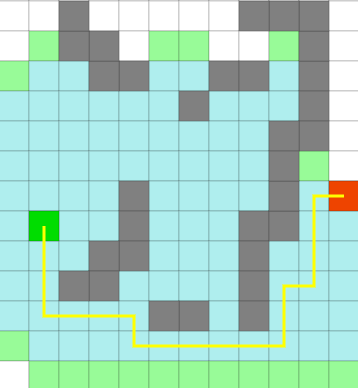
\includegraphics[width=0.5\textwidth]{figures/grid-astar.png}
        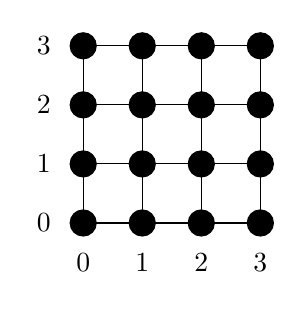
\begin{tikzpicture}[scale=0.5]
          % Grid pathfinding

\foreach \x in {0,...,3}
  \foreach \y in {0,...,3}
    {\node [draw, circle, fill=black] (\x\y) at (1.5*\x, 1.5*\y) {};}

\foreach \x in {0,...,3}
  \foreach \y in {0,...,2}
           {\draw (1.5 * \x, 1.5 * \y) -- (1.5 * \x, 1.5 * \y + 1.5);}

\foreach \y in {0,...,3}
  \foreach \x in {0,...,2}
           {\draw (1.5 * \x, 1.5 * \y) -- (1.5 * \x + 1.5, 1.5 * \y);}
           
\foreach \x in {0,...,3}
         {\node at (1.5 * \x, -1) {\x};
          \node at (-1, 1.5 * \x) {\x};
         }

        \end{tikzpicture}
	\caption{グリッド経路探索問題}
	\label{fig:grid-pathfinding}
\end{figure}


Web上に簡単に試せるデモがあるので、参照されたい\footnote{\url{http://qiao.github.io/PathFinding.js/visual/}}。この本で説明する様々なグラフ探索手法をグリッド経路探索に試すことが出来る。% この本の画像の一部はこのデモをもとに作成している。

グリッド経路探索はロボットのモーションプランニングやゲームAIなどで応用される\cite{algfoor2015comprehensive}。ストラテジーゲームなどでユニット(エージェント)を動かすために使われる \cite{cui2011based,sturtevant2012benchmarks}。% よく使われるベンチマーク問題集にもStarcraftのゲームのマップが含まれている\cite{sturtevant2012benchmarks}.
またグリッドは様々な問題を経路探索に帰着して解くことができるという意味でも重要である。例えば多重整列問題 (Multiple Sequence Alignment)はグリッド経路探索に帰着して解くことが出来る(節 \ref{sec:msa})。
ロボットのモーションプランニングも経路探索問題に帰着することが出来ることがある \cite{barraquand91}。$k$個の関節の角度を変えながら、現在状態から目的の状態 (Configuration)に近づけたい。各関節の角度をグリッドの各次元で表す。ロボットの物理的な構造のために不可能な角度の組み合わせを障害物の置かれたグリッドとする。このようにモデルを作ると、グリッド上で障害物を避けた経路を計算することで現在状態から目的状態へ関節をうまく動かすモーションプランが発見できる。

グリッド経路探索問題は重要な問題なのでさまざまな特化アルゴリズムが提案されている \cite{harabor2011online,bjornsson2003comparison,rabin2016combining,rivera2017grid}。例えばJump Point Searchは探索に意味のある中間地点 (Jump Point)を発見し探索を効率化する手法である \cite{harabor2014improving}。

\subsection{スライディングタイル (Sliding-tile Puzzle)}

多くの一人ゲームはグラフ探索問題に帰着することが出来る。スライディングタイルはその例であり、ヒューリスティック探索研究においてメジャーなベンチマーク問題でもある (図\ref{fig:15-puzzle}) \cite{johnson1879notes}。
$1$から$(n^2)-1$までの数字が振られたタイルが$n\times n$の正方形に並べられている。正方形には一つだけ{\it ブランク}と呼ばれるタイルのない位置があり、四方に隣り合うタイルのいずれかをその位置に移動する(スライドする)ことが出来る。スライディングタイル問題は、与えられた初期状態からスライドを繰り返し、ゴール状態にたどり着く経路を求める問題である。

\begin{figure}
\centering
% 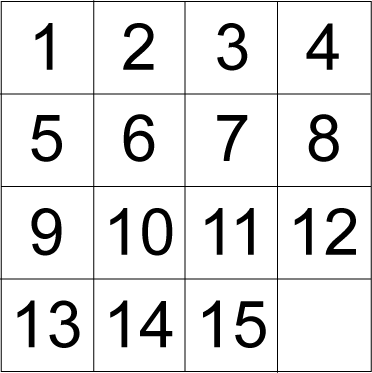
\includegraphics[bb=0 0 372 373,width=0.5\textwidth]{figures/15-puzzle.png}
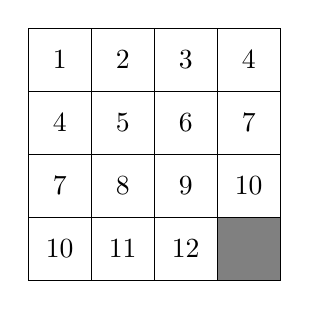
\begin{tikzpicture}[scale=0.8]
  % Sliding tile puzzle

\draw (0, 0) grid (4, 4);

\foreach \x in {0,...,3}
  \foreach \y in {0,...,3}
  {
        \pgfmathsetmacro{\val}{int(\x+3*\y+1)}
        \ifthenelse{\x=3 \AND \y=3}{;}{
          \node at (\x + 0.5, 3 - \y + 0.5) {\val};
        }
  }

\draw[fill=gray] (3,0) rectangle (4, 1);

\end{tikzpicture}
\caption{15パズルのゴール状態の例}
\label{fig:15-puzzle}
\end{figure}


スライディングタイルの到達可能な状態の数は$|V| = (n^2)!/2$\footnote{スライディングタイルは偶奇性があり、到達不可能な状態がある\cite{johnson1879notes}。}であり、$n$に対して指数的に増加する。
可能なアクションは$A= \{up, down, left, right\}$の4つであり、アクションにかかるコストはすべて同じとする。

後述するが、ヒューリスティック探索のためには状態からゴール状態までの距離(コスト)の下界(lower bound)が計算できると有用である。
スライディングタイルにおける下界の求め方として最もシンプルなものは{\it マンハッタン距離ヒューリスティック}である。マンハッタン距離ヒューリスティックは各タイルの現在状態の位置とゴール状態の位置のマンハッタン距離の総和を取る。可能なアクションはすべて一つしかタイルを動かさないので、一回のアクションでマンハッタン距離は最大で1しか縮まらない。よって、マンハッタン距離はゴールまでの距離の下界である。

%ちなみに、スライディングタイルはpermutation problemの一つである。

\subsection{多重整列問題 (Multiple Sequence Alignment)}
\label{sec:msa}
生物学・進化学では遺伝子配列・アミノ酸配列の編集距離(edit distance)を比較することでニ個体がどれだけ親しいかを推定することが広く研究されている。
\define{多重整列問題}{Multiple Sequence Alignment}{たじゅうせいれつもんだい} (MSA)は複数の遺伝子・アミノ酸配列が与えられた時、それらの配列間の編集距離とその時出来上がった配列を求める問題である \cite{corpet1988multiple}。
2つの配列に対してそれぞれコストの定義された編集操作を繰り返し、同一の配列に並べ替える手続きをアライメントと呼ぶ。
2つの配列の\define{編集距離}{edit distance}{へんしゅうきょり}は編集操作の合計コストの最小値である。
3つ以上の配列における距離の定義は様々考えられるが、例えば全ての配列のペアの編集距離の総和を用いられる。

MSAにおける可能な編集操作は置換と挿入である。置換は配列のある要素(DNAかアミノ酸)を別の要素に入れ替える操作であり、挿入は配列のある位置に要素を挿入する操作である。例えば(ATG, TGC, AGC)の3つの配列のアライメントを考える。表\ref{tbl:msa-cost}は置換と編集に対するコストの例である。-は欠損を示し、対応する要素が存在しないことを表す。% アミノ酸配列における有名なコスト表としてPAM250\cite{pearson1990}があるが、ここでは簡単のため仮のコスト表を用いる。
表\ref{tbl:msa}はこのコスト表を用いたアライメントの例である。
このとき、例えば配列ATG-と-TGCの編集距離は(A,-)、 (T,T)、 (G,G)、 (-,C)のコストの総和であるので、表\ref{tbl:msa-cost}を参照し、$3+0+0+3=6$である。同様に(ATG-, A-GC)の距離は$9$, (-TGC, A-GC)の距離は$6$であるので、3配列の編集距離は$6+9+6=21$である。

$n$配列のMSAは$n$次元のグリッドの経路探索問題に帰着することが出来る\cite{korf:2000}。
図\ref{tbl:msa-to-grid}は(ATG)と(TGC)の2つの配列によるMSAをグリッド経路探索問題に帰着した例である。
状態$s = (x_1, x_2,...,x_n)$の各変数$x_i$は配列$i$のどの位置までアライメントを完了したかを表す変数であり、配列$i$の長さを$l_i$とすると定義域は$0 \leq x_0 \leq l_0$である。
全てのアライメントが完了した状態$s=(l_1, l_2,...,l_n)$がゴール状態である。
可能なアクション$a=(b_1, b_2, ..., b_n), (b_i=0, 1)$は配列$i$に対してそれぞれ欠損を挿入するか否かであり、配列$i$に対して欠損を挿入する場合に$b_i=0$、挿入しない場合は$b_i=1$となる。
状態$s$に対してアクション$a$を適用した後の状態$s'$は$s'=(x_1+b_1, x_2+b_2,..., x_n+b_n)$となる。図\ref{tbl:msa-to-grid}は初期状態$s=(0,0)$に対して$a=(1,0)$を適用している。これは(A), (-)までアライメントを進めた状態に対応する。次に$a=(1,1)$が適用され、アライメントは(A,T), (-,T)という状態に遷移する。このようにして$(0, 0)$から$(l_1, l_2)$までたどり着くまでの最小コストを求める。

MSAは可能なアクションの数が配列の数$n$に対して指数的に増える ($2^n-1$)点が難しい。アミノ酸配列が対象である場合はコストの値が幅広い点も難しい \cite{pearson1990}。
MSAは生物学研究に役立つというモチベーションから非常に熱心に研究されており、様々な定式化による解法が知られている。
詳しくは\cite{waterman1995introduction,
gusfield1997algorithms,edgar2006multiple}を参照されたい。

\begin{table}
  \centering
  \caption{多重配列問題 (MSA)}
  \begin{tabular}{c|cccc}
    \toprule
	Sequence1 & A & T & G & - \\
	Sequence2 & - & T & G & C \\
	Sequence3 & A & - & G & C \\
        \bottomrule
\end{tabular}
\label{tbl:msa}
\end{table}

\begin{table}
  \centering
\caption{MSAの塩基配列のコスト表}
\begin{tabular}{c|ccccc}
  \toprule
	  & A & T & G & C & - \\ \midrule
	A & 0 & 3 & 3 & 3 & 3 \\
	T & 3 & 0 & 3 & 3 & 3 \\
	G & 3 & 3 & 0 & 3 & 3 \\
	C & 3 & 3 & 3 & 0 & 3 \\
	- & 3 & 3 & 3 & 3 & 0 \\
        \bottomrule
\end{tabular}
\label{tbl:msa-cost}
\end{table}

\begin{table}
  \centering
\caption{MSAのグリッド経路探索問題への帰着}
\begin{tabular}{c|cccc}
  \toprule
	  & A & T & G & - \\ \midrule
	T & $\rightarrow$ & $\searrow$ &   &   \\
	G &   &   & $\searrow$ &   \\
	C &   &   &   & $\downarrow$ \\
        \bottomrule
\end{tabular}
\label{tbl:msa-to-grid}
\end{table}


\subsection{倉庫番 (Sokoban)}
倉庫番(Sokoban)は倉庫の荷物を押していくことで指定された位置に置くというパズルゲームである。現在でも様々なゲームの中で親しまれている \cite{junghanns1997sokoban,culberson:97}。
プレイヤーは「荷物の後ろに回って押す」ことしか出来ず、引っ張ったり、横から動かしたりすることが出来ない。また、荷物の上を通ることも出来ない。
このシンプルなルールのパズルはPSPACE-completeであることが知られている\cite{culberson:97}。

%     ####
% #####  #
% #   $  #
% #  .#  #
% ## ## ##
% #      #
% # @#   #
% #  #####
% ####

\begin{figure}
\centering
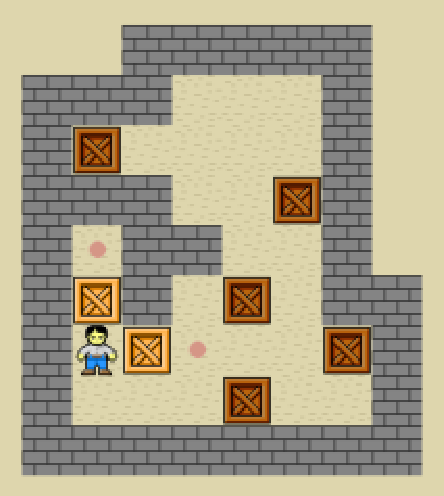
\includegraphics[width=0.4\textwidth]{figures/sokoban.pdf}
\caption{倉庫番 (画像はWikipediaより)}
\label{fig:sokoban}
\end{figure}

状態の表現方法は2通りあり、一つはグリッドの各位置に何が置いてあるかを変数とする方法である。もうひとつはプレイヤー、各荷物の位置に対してそれぞれ変数を割り当てる方法である。
可能なアクションは{\tt move-up}, {\tt move-left}, {\tt move-down}, {\tt move-right}, {\tt push-up}, {\tt push-left}, {\tt push-down}, {\tt push-right} の8通りである。{\tt move-*}はプレイヤーが動くアクションに対応し、コストは0である。{\tt push-*}は荷物を押すアクションであり、正のアクションコストが割当てられている。よって、倉庫番はなるべく荷物を押す回数を少なくして荷物を目的の位置に動かすことが目的となる。

グラフ探索問題として倉庫番を考えるときに重要であるのは、倉庫番は\define{不可逆なアクション}{irreversible action}{ふかぎゃくなアクション}が存在することである。
全てのアクション$a \in A$に対して$a^{-1} \in A$が存在し、$a(a^{-1}(s)) = s$かつ$a^{-1}(a(s)) = s$となる場合、問題は\define{可逆}{reversible}{かぎゃく}であると呼ぶ。
例えばグリッド経路探索やスライディングタイルは可逆である。
可逆な問題は対応するアクションのコストが同じであれば無向グラフとしてモデルすることもでき、初期状態から到達できる状態は、すべて初期状態に戻ることが出来る。
一方、不可逆な問題ではこれが保証されず、デッドエンドにはまる可能性がある (\ref{sec:difficulity}節)。

倉庫番では荷物を押すことは出来ても引っ張ることが出来ないため、不可逆な問題である。例えば、荷物を部屋の隅に置いてしまうと戻すことが出来ないため、詰み状態 (dead end)に陥る可能性がある問題である。
このような性質を持つ問題では特にグラフ探索による先読みが効果的である。

倉庫番のもうひとつ重要な性質は\define{ゼロコストアクション}{zero-cost action}{ゼロコストアクション}の存在である。ゼロコストアクションはコストが0のアクションである \cite{asai2016tiebreaking}。
倉庫番のアクションのうち{\tt move-up}, {\tt move-left}, {\tt move-down}, {\tt move-right}はコストゼロ($w(a)=0$)のアクションである。ヘタなアルゴリズムを実行すると無限に無駄なアクションを繰り返し続けるということもありうる。


\subsection{巡回セールスパーソン問題 (Traveling Salesperson Problem, TSP)}

\begin{figure}
\centering
% 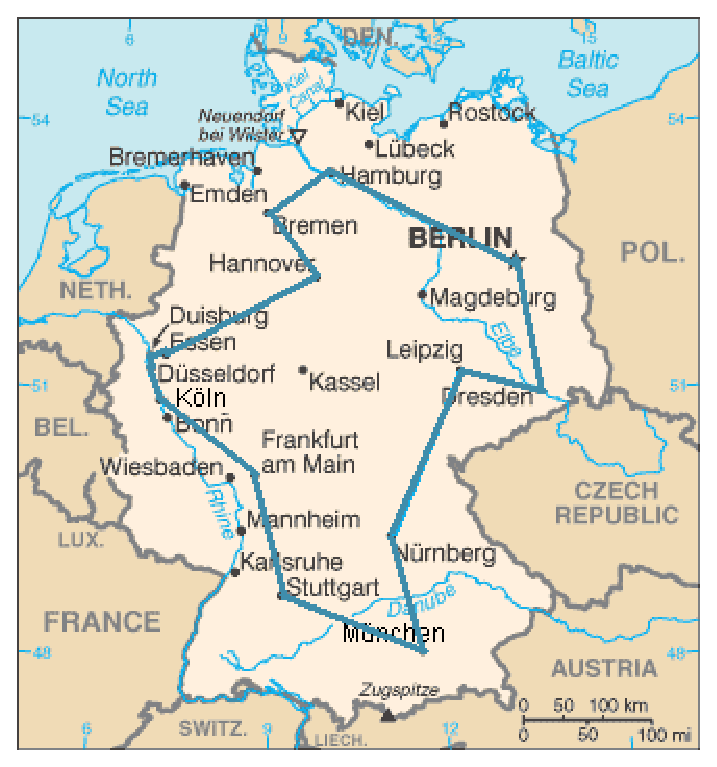
\includegraphics[bb=0 0 328 352,width=0.5\textwidth]{figures/tsp.eps}%TODO 
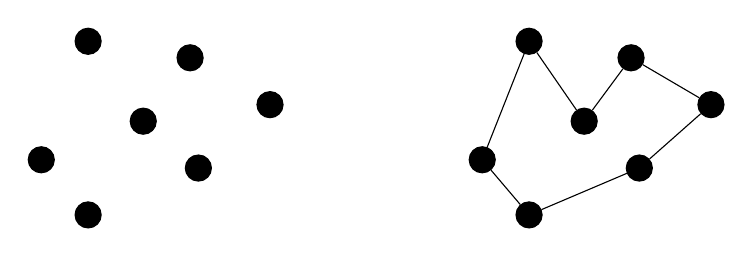
\begin{tikzpicture}[scale=0.7]
  \foreach \x in {0, 8}
  {
    \pgfmathsetmacro{\noise}{0.15}           
\node[draw,circle,fill=black] (1\x) at (\x+0, 0) {};
\node[draw,circle,fill=black] (2\x) at (\x+2, 1-\noise) {};
\node[draw,circle,fill=black] (3\x) at (\x+3+2*\noise, 2) {};
\node[draw,circle,fill=black] (4\x) at (\x+2-\noise, 3-\noise) {};
\node[draw,circle,fill=black] (5\x) at (\x+1, 2-2*\noise) {};
\node[draw,circle,fill=black] (6\x) at (\x+0, 3+\noise) {};
\node[draw,circle,fill=black] (7\x) at (\x-1+\noise, 1) {};
}

\foreach \a in {1,...,6}
  {
    \pgfmathsetmacro{\n}{int(\a+1)}
    \draw[-] (\a8) -- (\n8);
  }

\draw[-] (78) -- (18);

\end{tikzpicture}
\caption{巡回セールスパーソン問題}
\label{fig:sokoban}
\end{figure}


巡回セールスパーソン問題は、地図上にある都市を全て回り最初の都市に戻るときの最短距離の経路を求める問題である \cite{applegate2006traveling}。
$n$個の都市があるとすると(非最適解含む)解の数は$(n-1)!/2$個である。
可能なアクションは「都市$i \in \{1..n\}$を訪れる」であり、一度訪れた都市には行けない。
TSPのゴール条件はすべての都市を訪れることである。よって、何も考えずに$n$回アクションを実行すれば、とりあえず解を得ることが出来る。しかし最適解を得ることは難しく、NP完全問題であることが知られている。
TSPはヒューリスティック探索に限らず、様々なアプローチで研究されている実用的に非常に重要なドメインである\cite{applegate2006traveling}。TSPについて特に詳しく知りたい方はそちらの教科書を参照されたい。


\section{問題の性質・難しさ}
\label{sec:difficulity}

本書で定義した状態空間問題は小さなモデルである。このモデルは完全情報であり、状態遷移は決定論的である。
それでも状態空間問題の最小コスト経路を発見する問題はNP困難である。
このように一般には難しい問題でも、後述するヒューリスティック探索で解けるかもしれない。
問題の難しさを定量化することは難しく、さまざまなアプローチが研究されている \cite{wilt2012does,xie2015understanding,cohen2017problem,backstrom2017time}。

この節では問題の難しさを測るための判断材料を列挙する。

\begin{enumerate}
\item {\bf 状態空間の大きさ}

状態空間の大きさ$|S|$は大きい程概して問題は難しくなる。
特に状態空間が無限である場合深さ優先探索などのアルゴリズムは停止しない場合がある。
例えば状態変数に実数が含まれる場合、状態空間の大きさは無限になる。
% 状態空間の大きさがそのまま問題の難しさに直結するわけではない。

\item {\bf 分枝度}

ある状態$s$の\define{分枝度}{branching factor}{ぶんしど}はそのノードの子ノードの数を指す。
特に状態空間問題の分枝度は、すべての状態の分枝度の平均を指す。ただし多くの場合平均を厳密に求めることはなく、おおよその平均を指して分枝度をすることが多い。
分枝度が大きいほど問題は難しいとは限らない。
分枝度が多いほどグラフが密である、つまりエッジの数が多いことに対応する \cite{cohen2017problem}。
%エッジが多い程解の候補となる経路が多くなる。
分枝度を$b$とすると、あるノード$s$の子ノードの数は$b$個であり、孫ノードの数は$b^2$である。$s$からの深さ$d$のノードは$b^d$個である。

\item {\bf デッドエンド}

問題によってはある状態に到達するともう問題を解くことは出来ないというシチュエーションがある。例えば倉庫番は荷物を角においてしまうともう動かすことができない。これによってもう問題がクリアできなくなるということがある。このような問題では状態空間を広く探索し、デッドエンド状態のみを探索し続けるということをうまく避ける必要がある。例えば\ref{sec:greedy-best-first-search}節の貪欲最良優先探索はデッドエンドに入ってしまうとなかなか抜け出せないかもしれない。
% あるいはデッドエンドを検知する手法も考えられる。
概してデッドエンドがある問題では状態空間を広く探索する手法、探索済みの状態を記録する手法が有利であり、局所探索手法はうまくいかないことがある。
%このような問題では局所探索アルゴリズムではうまくいかないことがある。局所探索アルゴリズムは

\item {\bf 解の存在}

当然解が存在しない問題もありうる。
本書で紹介するアルゴリズムは解が存在しない場合非常に時間がかかるものが多い\footnote{一般にどのようなアルゴリズムを使っても解が存在しない状態空間問題は難しい。}。
一部のアルゴリズムは解が存在しない場合永遠に停止しない場合がある。
そのような場合、アルゴリズムは解が存在しないと示せれば理想的である。
そのため解が存在しないことを検出するアルゴリズムの研究もされている \cite{backstrom2013fast,hoffmann2014distance}。

\end{enumerate}

\section{関連文献}

本章で扱うヒューリスティック探索は主にここで定義した状態空間問題への適用を前提として書かれている。
そのため状態空間問題よりも広い問題を解くためには少し工夫が必要になることが多い。

状態空間問題は完全情報であり状態遷移が決定論的であることを仮定した。
状態遷移が決定論的ではなく確率的であると仮定したモデルは\define{マルコフ過程問題}{Markov Decision Process Problem}{マルコフかていもんだい} (MDP)と呼ばれている \cite{puterman2014markov}。
MDP$(S, A, P, R)$は状態集合$S$、アクション集合$A$、状態遷移確率$P$、報酬$R$からなる。
状態空間問題は状態遷移が決定論的であるのに対してMDPのそれは確率的である。
また、MDPはコストを最小化するのではなく報酬の総和の期待値を最大化する問題として定義されることが多い。
状態空間問題はMDPのうち状態遷移が常に決定的であるものである。
MDPは\define{強化学習}{reinforcement learning}{きょうかがくしゅう}における問題モデルとしても広く使われている \cite{sutton:99}。
状態遷移が決定論的であれば、状態遷移は一つの状態から一つの状態へのエッジによって表すことができる。状態遷移が確率的である場合は可能な次状態を列挙するAND-OR木 \cite{luger1997artificial}でモデルすることが出来る。
MDPを解くには動的計画法 \cite{puterman2014markov,barto1995learning}やモンテカルロ木探索 \cite{browne2012survey,kocsis2006bandit}が使われることが多い。

MDPからさらに不完全情報問題に拡張したものを\define{部分観測マルコフ過程問題}{partially observable Markov decision process problem}{ぶぶんかんそくマルコフかていもんだい} (POMDP)と呼ぶ \cite{kaelbling1998planning}。
POMDPにおけるプランニング問題の厳密解はBelief space \cite{kaelbling1998planning}上を探索することで求められるが、多くの場合厳密計算は困難なのでモンテカルロ木探索などの近似手法が用いられる。
POMDPは非常に計算が難しいモデルであるので、仮にPOMDPが与えられた問題をもっとも正確に表せられるモデルであったとしても近似的にMDPを使った方がうまくいくかもしれない。

囲碁やチェスなどの敵対するエージェントがいる問題も探索が活躍するドメインであり、特に二人零和ゲームでの研究が盛んである。
このような問題では敵プレイヤーの取るアクションが事前に分からないのでAND-OR木でモデルすることが多い。
敵対ゲームを解くための手法としてはMiniMax木、$\alpha$-$\beta$木\cite{pearl84}やモンテカルロ木探索などがある。近年では強化学習によってヒューリスティック関数を学習するアプローチが盛んに研究されている \cite{sutton:99}。

ヒューリスティック探索はゲームやロボティクスの応用の中で現れる経路探索問題を解くために特によく使われる。
ゲームに探索を使う場合問題になるのは計算にかかる時間である。
たとえば次の一手を計算するために一日以上かかるチェスAIとプレイしたい人は少ないだろう。
このような応用では解のコストだけでなく、解を得るために使う時間も評価しなければならない。
このような問題をリアルタイム探索と呼ぶ \cite{korf90,barto1995learning}。
リアルタイム探索にはLearning real-time A* (LRTA*) \cite{korf90,koenig2001minimax}やReal-time adaptive A* (RTAA*) \cite{koenig2006real}などが使われる。

本書ではノードの次数が有限 (局所有限グラフ)である問題を対象としたアルゴリズムを紹介している。
一見自然な仮定だが、この仮定ではアクションや状態空間の大きさが無限である連続空間問題を解くことができない。そのためロボティクスで現れる連続空間問題を解くためには工夫が必要になる。
例えばグリッド経路探索問題で任意の角度を取ることが出来るAny-angle path planning問題は本書では扱わないが、ヒューリスティック探索の派生アルゴリズムで解くことができる\cite{lavalle2006planning,lavalle2001rapidly,daniel2010theta,nash2013any}。

状態空間問題は制約充足問題の一種であり、例えばBoolean satisfiability problem (SAT)として書くことができる \cite{garey1979computers}。それを利用してSATによって状態空間問題を解くアプローチも広く研究されている \cite{kautz1992planning,kautz2006satplan,rintanen2012planning}。状態空間問題では表現することが難しい制約や目的関数がある場合は制約充足問題や離散最適化問題としてモデルすることもできる。
